\documentclass{beamer}
\usetheme{Madrid}
\usecolortheme{seagull}
\usepackage[utf8]{inputenc}
\usepackage[russian]{babel}
\usepackage{graphicx}

% Информация о презентации
\title[Цветовые гармонии]{Цветовые гармонии и их применение}
\author[Ф. А. Мусатов]{Исполнитель: студент группы 221 факультета КНиИТ \\ Ф. А. Мусатов \\ Руководитель НИР: старший преподаватель М. В. Белоконь}
\institute[Саратов]{Саратовский государственный университет}
\date{Саратов, 2024}

\begin{document}

% Титульный слайд
\begin{frame}
    \titlepage
\end{frame}

% Слайд 1: Аналоговая гармония
\begin{frame}{Аналоговая гармония}
    \textbf{Определение:} Сочетание цветов, расположенных рядом на цветовом круге. \\
    \vspace{0.3cm}
    \textbf{Эффект:} Создаёт мягкие и спокойные композиции. \\
    \vspace{0.3cm}
    \textbf{Применение:} Пейзажи, интерьер для создания уюта и гармонии.
    \begin{center}
        
\includegraphics[width=0.6\linewidth]{analog_example.png} % Замените на реальное изображение
    \end{center}
\end{frame}

% Слайд 2: Родственноконтрастные цвета
\begin{frame}{Цветовая схема родственноконтрастных цветов}
    \textbf{Суть:} Оттенки с общим элементом, но разной насыщенностью или светлотой. \\
    \vspace{0.3cm}
    \textbf{Эффект:} Контраст без резких конфликтов. \\
    \vspace{0.3cm}
    \textbf{Применение:} Модные коллекции, элегантный интерьер.
    \begin{center}
        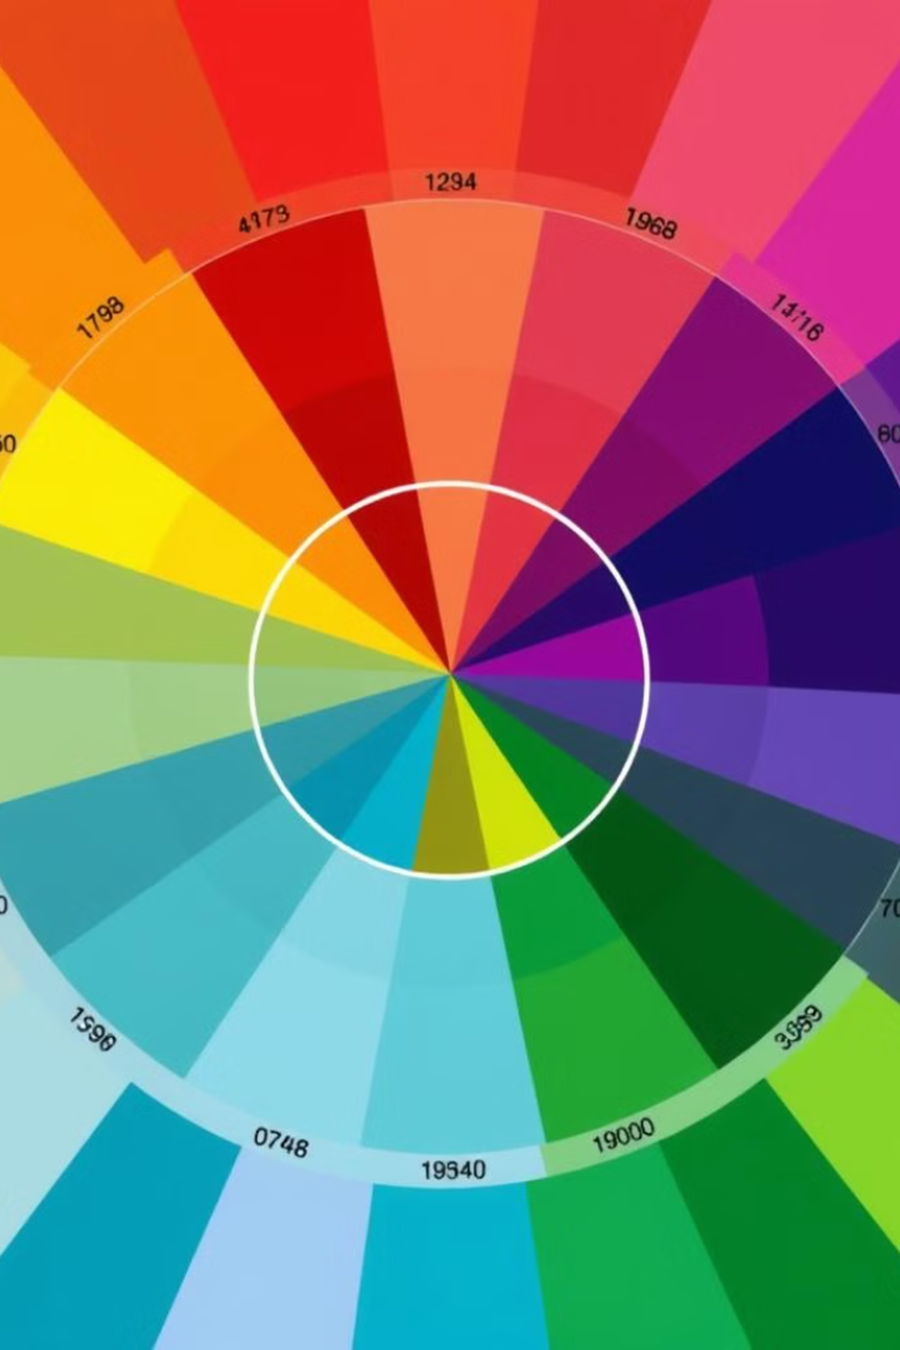
\includegraphics[width=0.6\linewidth]{related_contrast_example.png} % Замените на реальное изображение
    \end{center}
\end{frame}

% Слайд 3: Контрастные цвета
\begin{frame}{Цветовая схема контрастных цветов}
    \textbf{Определение:} Цвета на противоположных сторонах цветового круга. \\
    \vspace{0.3cm}
    \textbf{Эффект:} Сильная динамика, привлечение внимания. \\
    \vspace{0.3cm}
    \textbf{Применение:} Реклама, графический дизайн.
    \begin{center}
        
\includegraphics[width=0.6\linewidth]{contrast_example.png} % Замените на реальное изображение
    \end{center}
\end{frame}

% Слайд 4: Комплементарные цвета
\begin{frame}{Комплементарные цвета}
    \textbf{Определение:} Дополняют друг друга, создавая яркий контраст. \\
    \vspace{0.3cm}
    \textbf{Эффект:} Привлекают внимание и придают глубину. \\
    \vspace{0.3cm}
    \textbf{Применение:} Живопись, дизайн интерьеров.
    \begin{center}
        
\includegraphics[width=0.6\linewidth]{complementary_example.png} % Замените на реальное изображение
    \end{center}
\end{frame}

% Слайд 5: Триадные гармонические схемы
\begin{frame}{Триадные гармонические схемы}
    \textbf{Выбор цветов:} Три цвета, равномерно расположенные на цветовом круге. \\
    \vspace{0.3cm}
    \textbf{Эффект:} Динамическое равновесие, выразительные композиции. \\
    \vspace{0.3cm}
    \textbf{Применение:} Логотипы для передачи разнообразия.
    \begin{center}
        
\includegraphics[width=0.6\linewidth]{triadic_example.png} % Замените на реальное изображение
    \end{center}
\end{frame}

% Слайд 6: Источники
\begin{frame}{Список использованных источников}
    \begin{itemize}
        \item Альберс Й. Interaction of Color. Yale University Press, 1971.
        \item Тернбулл Д. Color: A Natural History of the Palette. Random House, 2004.
        \item Альберс Й. The Art of Color. Yale University Press, 1975.
        \item Гурни Дж. Color and Light: A Guide for the Realist Painter. Andrews McMeel Publishing, 2010.
        \item Adobe. Adobe Color Wheel [Электронный ресурс]. Доступно на: \url{https://color.adobe.com}.
    \end{itemize}
\end{frame}

% Слайд 7: Спасибо за внимание
\begin{frame}
    \centering
    \textbf{\huge Спасибо за внимание!}
\end{frame}

\end{document}
